% Created by tikzDevice version 0.12.6 on 2025-04-07 03:13:54
% !TEX encoding = UTF-8 Unicode
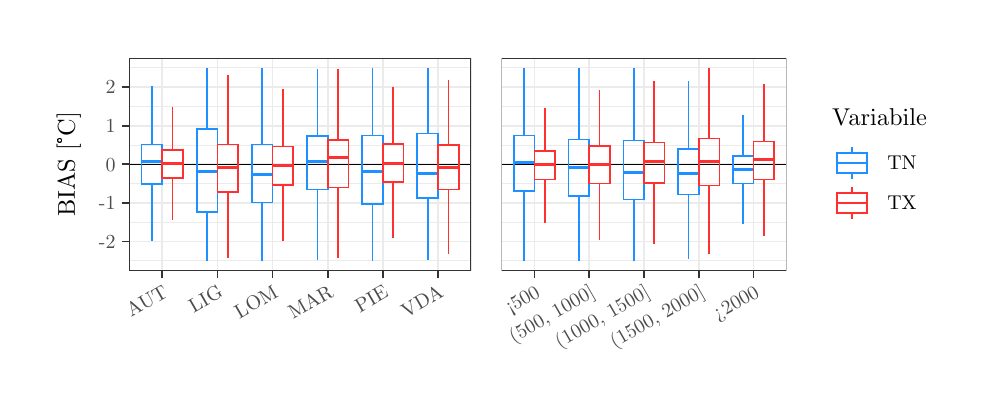
\begin{tikzpicture}[x=1pt,y=1pt]
\definecolor{fillColor}{RGB}{255,255,255}
\path[use as bounding box,fill=fillColor] (0,0) rectangle (341.43,128.04);
\begin{scope}
\path[clip] (  0.00,  0.00) rectangle (341.43,128.04);
\definecolor{drawColor}{RGB}{255,255,255}

\path[draw=drawColor,line width= 0.6pt,line join=round,line cap=round,fill=fillColor] (  0.00,  0.00) rectangle (341.43,128.04);
\end{scope}
\begin{scope}
\path[clip] (  5.50,  5.50) rectangle (165.73,122.54);
\definecolor{drawColor}{RGB}{255,255,255}
\definecolor{fillColor}{RGB}{255,255,255}

\path[draw=drawColor,line width= 0.6pt,line join=round,line cap=round,fill=fillColor] (  5.50,  5.50) rectangle (165.73,122.54);
\end{scope}
\begin{scope}
\path[clip] (165.73,  5.50) rectangle (335.93,122.54);
\definecolor{drawColor}{RGB}{255,255,255}
\definecolor{fillColor}{RGB}{255,255,255}

\path[draw=drawColor,line width= 0.6pt,line join=round,line cap=round,fill=fillColor] (165.73,  5.50) rectangle (335.93,122.54);
\end{scope}
\begin{scope}
\path[clip] ( 36.68, 40.29) rectangle (160.23,117.04);
\definecolor{fillColor}{RGB}{255,255,255}

\path[fill=fillColor] ( 36.68, 40.29) rectangle (160.23,117.04);
\definecolor{drawColor}{gray}{0.92}

\path[draw=drawColor,line width= 0.3pt,line join=round] ( 36.68, 43.78) --
	(160.23, 43.78);

\path[draw=drawColor,line width= 0.3pt,line join=round] ( 36.68, 57.73) --
	(160.23, 57.73);

\path[draw=drawColor,line width= 0.3pt,line join=round] ( 36.68, 71.69) --
	(160.23, 71.69);

\path[draw=drawColor,line width= 0.3pt,line join=round] ( 36.68, 85.64) --
	(160.23, 85.64);

\path[draw=drawColor,line width= 0.3pt,line join=round] ( 36.68, 99.59) --
	(160.23, 99.59);

\path[draw=drawColor,line width= 0.3pt,line join=round] ( 36.68,113.55) --
	(160.23,113.55);

\path[draw=drawColor,line width= 0.6pt,line join=round] ( 36.68, 50.75) --
	(160.23, 50.75);

\path[draw=drawColor,line width= 0.6pt,line join=round] ( 36.68, 64.71) --
	(160.23, 64.71);

\path[draw=drawColor,line width= 0.6pt,line join=round] ( 36.68, 78.66) --
	(160.23, 78.66);

\path[draw=drawColor,line width= 0.6pt,line join=round] ( 36.68, 92.62) --
	(160.23, 92.62);

\path[draw=drawColor,line width= 0.6pt,line join=round] ( 36.68,106.57) --
	(160.23,106.57);

\path[draw=drawColor,line width= 0.6pt,line join=round] ( 48.64, 40.29) --
	( 48.64,117.04);

\path[draw=drawColor,line width= 0.6pt,line join=round] ( 68.56, 40.29) --
	( 68.56,117.04);

\path[draw=drawColor,line width= 0.6pt,line join=round] ( 88.49, 40.29) --
	( 88.49,117.04);

\path[draw=drawColor,line width= 0.6pt,line join=round] (108.42, 40.29) --
	(108.42,117.04);

\path[draw=drawColor,line width= 0.6pt,line join=round] (128.35, 40.29) --
	(128.35,117.04);

\path[draw=drawColor,line width= 0.6pt,line join=round] (148.27, 40.29) --
	(148.27,117.04);
\definecolor{drawColor}{RGB}{0,0,0}

\path[draw=drawColor,line width= 0.1pt,line join=round] ( 36.68, 78.66) -- (160.23, 78.66);
\definecolor{drawColor}{RGB}{30,144,255}

\path[draw=drawColor,line width= 0.6pt,line join=round] ( 44.90, 85.77) -- ( 44.90,106.91);

\path[draw=drawColor,line width= 0.6pt,line join=round] ( 44.90, 71.66) -- ( 44.90, 50.99);

\path[draw=drawColor,line width= 0.6pt] ( 41.17, 85.77) --
	( 41.17, 71.66) --
	( 48.64, 71.66) --
	( 48.64, 85.77) --
	( 41.17, 85.77) --
	cycle;

\path[draw=drawColor,line width= 1.1pt] ( 41.17, 79.51) -- ( 48.64, 79.51);
\definecolor{drawColor}{RGB}{255,48,48}

\path[draw=drawColor,line width= 0.6pt,line join=round] ( 52.37, 83.94) -- ( 52.37, 99.20);

\path[draw=drawColor,line width= 0.6pt,line join=round] ( 52.37, 73.76) -- ( 52.37, 58.64);

\path[draw=drawColor,line width= 0.6pt] ( 48.64, 83.94) --
	( 48.64, 73.76) --
	( 56.11, 73.76) --
	( 56.11, 83.94) --
	( 48.64, 83.94) --
	cycle;

\path[draw=drawColor,line width= 1.1pt] ( 48.64, 78.89) -- ( 56.11, 78.89);
\definecolor{drawColor}{RGB}{30,144,255}

\path[draw=drawColor,line width= 0.6pt,line join=round] ( 64.83, 91.37) -- ( 64.83,113.45);

\path[draw=drawColor,line width= 0.6pt,line join=round] ( 64.83, 61.54) -- ( 64.83, 43.82);

\path[draw=drawColor,line width= 0.6pt] ( 61.09, 91.37) --
	( 61.09, 61.54) --
	( 68.56, 61.54) --
	( 68.56, 91.37) --
	( 61.09, 91.37) --
	cycle;

\path[draw=drawColor,line width= 1.1pt] ( 61.09, 76.14) -- ( 68.56, 76.14);
\definecolor{drawColor}{RGB}{255,48,48}

\path[draw=drawColor,line width= 0.6pt,line join=round] ( 72.30, 85.77) -- ( 72.30,110.93);

\path[draw=drawColor,line width= 0.6pt,line join=round] ( 72.30, 68.70) -- ( 72.30, 44.93);

\path[draw=drawColor,line width= 0.6pt] ( 68.56, 85.77) --
	( 68.56, 68.70) --
	( 76.04, 68.70) --
	( 76.04, 85.77) --
	( 68.56, 85.77) --
	cycle;

\path[draw=drawColor,line width= 1.1pt] ( 68.56, 77.43) -- ( 76.04, 77.43);
\definecolor{drawColor}{RGB}{30,144,255}

\path[draw=drawColor,line width= 0.6pt,line join=round] ( 84.76, 85.85) -- ( 84.76,113.35);

\path[draw=drawColor,line width= 0.6pt,line join=round] ( 84.76, 64.85) -- ( 84.76, 43.82);

\path[draw=drawColor,line width= 0.6pt] ( 81.02, 85.85) --
	( 81.02, 64.85) --
	( 88.49, 64.85) --
	( 88.49, 85.85) --
	( 81.02, 85.85) --
	cycle;

\path[draw=drawColor,line width= 1.1pt] ( 81.02, 75.02) -- ( 88.49, 75.02);
\definecolor{drawColor}{RGB}{255,48,48}

\path[draw=drawColor,line width= 0.6pt,line join=round] ( 92.23, 85.11) -- ( 92.23,105.83);

\path[draw=drawColor,line width= 0.6pt,line join=round] ( 92.23, 71.29) -- ( 92.23, 50.81);

\path[draw=drawColor,line width= 0.6pt] ( 88.49, 85.11) --
	( 88.49, 71.29) --
	( 95.96, 71.29) --
	( 95.96, 85.11) --
	( 88.49, 85.11) --
	cycle;

\path[draw=drawColor,line width= 1.1pt] ( 88.49, 78.12) -- ( 95.96, 78.12);
\definecolor{drawColor}{RGB}{30,144,255}

\path[draw=drawColor,line width= 0.6pt,line join=round] (104.68, 88.87) -- (104.68,113.21);

\path[draw=drawColor,line width= 0.6pt,line join=round] (104.68, 69.52) -- (104.68, 44.06);

\path[draw=drawColor,line width= 0.6pt] (100.95, 88.87) --
	(100.95, 69.52) --
	(108.42, 69.52) --
	(108.42, 88.87) --
	(100.95, 88.87) --
	cycle;

\path[draw=drawColor,line width= 1.1pt] (100.95, 79.85) -- (108.42, 79.85);
\definecolor{drawColor}{RGB}{255,48,48}

\path[draw=drawColor,line width= 0.6pt,line join=round] (112.16, 87.44) -- (112.16,113.05);

\path[draw=drawColor,line width= 0.6pt,line join=round] (112.16, 70.32) -- (112.16, 44.92);

\path[draw=drawColor,line width= 0.6pt] (108.42, 87.44) --
	(108.42, 70.32) --
	(115.89, 70.32) --
	(115.89, 87.44) --
	(108.42, 87.44) --
	cycle;

\path[draw=drawColor,line width= 1.1pt] (108.42, 81.21) -- (115.89, 81.21);
\definecolor{drawColor}{RGB}{30,144,255}

\path[draw=drawColor,line width= 0.6pt,line join=round] (124.61, 89.09) -- (124.61,113.35);

\path[draw=drawColor,line width= 0.6pt,line join=round] (124.61, 64.37) -- (124.61, 43.83);

\path[draw=drawColor,line width= 0.6pt] (120.87, 89.09) --
	(120.87, 64.37) --
	(128.35, 64.37) --
	(128.35, 89.09) --
	(120.87, 89.09) --
	cycle;

\path[draw=drawColor,line width= 1.1pt] (120.87, 76.15) -- (128.35, 76.15);
\definecolor{drawColor}{RGB}{255,48,48}

\path[draw=drawColor,line width= 0.6pt,line join=round] (132.08, 85.99) -- (132.08,106.52);

\path[draw=drawColor,line width= 0.6pt,line join=round] (132.08, 72.30) -- (132.08, 51.90);

\path[draw=drawColor,line width= 0.6pt] (128.35, 85.99) --
	(128.35, 72.30) --
	(135.82, 72.30) --
	(135.82, 85.99) --
	(128.35, 85.99) --
	cycle;

\path[draw=drawColor,line width= 1.1pt] (128.35, 78.91) -- (135.82, 78.91);
\definecolor{drawColor}{RGB}{30,144,255}

\path[draw=drawColor,line width= 0.6pt,line join=round] (144.54, 89.74) -- (144.54,113.51);

\path[draw=drawColor,line width= 0.6pt,line join=round] (144.54, 66.49) -- (144.54, 43.92);

\path[draw=drawColor,line width= 0.6pt] (140.80, 89.74) --
	(140.80, 66.49) --
	(148.27, 66.49) --
	(148.27, 89.74) --
	(140.80, 89.74) --
	cycle;

\path[draw=drawColor,line width= 1.1pt] (140.80, 75.18) -- (148.27, 75.18);
\definecolor{drawColor}{RGB}{255,48,48}

\path[draw=drawColor,line width= 0.6pt,line join=round] (152.01, 85.62) -- (152.01,109.24);

\path[draw=drawColor,line width= 0.6pt,line join=round] (152.01, 69.62) -- (152.01, 46.19);

\path[draw=drawColor,line width= 0.6pt] (148.27, 85.62) --
	(148.27, 69.62) --
	(155.75, 69.62) --
	(155.75, 85.62) --
	(148.27, 85.62) --
	cycle;

\path[draw=drawColor,line width= 1.1pt] (148.27, 77.50) -- (155.75, 77.50);
\definecolor{drawColor}{gray}{0.20}

\path[draw=drawColor,line width= 0.6pt,line join=round,line cap=round] ( 36.68, 40.29) rectangle (160.23,117.04);
\end{scope}
\begin{scope}
\path[clip] (  0.00,  0.00) rectangle (341.43,128.04);
\definecolor{drawColor}{gray}{0.30}

\node[text=drawColor,anchor=base east,inner sep=0pt, outer sep=0pt, scale=  0.72] at ( 31.73, 48.29) {-2};

\node[text=drawColor,anchor=base east,inner sep=0pt, outer sep=0pt, scale=  0.72] at ( 31.73, 62.25) {-1};

\node[text=drawColor,anchor=base east,inner sep=0pt, outer sep=0pt, scale=  0.72] at ( 31.73, 76.20) {0};

\node[text=drawColor,anchor=base east,inner sep=0pt, outer sep=0pt, scale=  0.72] at ( 31.73, 90.15) {1};

\node[text=drawColor,anchor=base east,inner sep=0pt, outer sep=0pt, scale=  0.72] at ( 31.73,104.11) {2};
\end{scope}
\begin{scope}
\path[clip] (  0.00,  0.00) rectangle (341.43,128.04);
\definecolor{drawColor}{gray}{0.20}

\path[draw=drawColor,line width= 0.6pt,line join=round] ( 33.93, 50.75) --
	( 36.68, 50.75);

\path[draw=drawColor,line width= 0.6pt,line join=round] ( 33.93, 64.71) --
	( 36.68, 64.71);

\path[draw=drawColor,line width= 0.6pt,line join=round] ( 33.93, 78.66) --
	( 36.68, 78.66);

\path[draw=drawColor,line width= 0.6pt,line join=round] ( 33.93, 92.62) --
	( 36.68, 92.62);

\path[draw=drawColor,line width= 0.6pt,line join=round] ( 33.93,106.57) --
	( 36.68,106.57);
\end{scope}
\begin{scope}
\path[clip] (  0.00,  0.00) rectangle (341.43,128.04);
\definecolor{drawColor}{gray}{0.20}

\path[draw=drawColor,line width= 0.6pt,line join=round] ( 48.64, 37.54) --
	( 48.64, 40.29);

\path[draw=drawColor,line width= 0.6pt,line join=round] ( 68.56, 37.54) --
	( 68.56, 40.29);

\path[draw=drawColor,line width= 0.6pt,line join=round] ( 88.49, 37.54) --
	( 88.49, 40.29);

\path[draw=drawColor,line width= 0.6pt,line join=round] (108.42, 37.54) --
	(108.42, 40.29);

\path[draw=drawColor,line width= 0.6pt,line join=round] (128.35, 37.54) --
	(128.35, 40.29);

\path[draw=drawColor,line width= 0.6pt,line join=round] (148.27, 37.54) --
	(148.27, 40.29);
\end{scope}
\begin{scope}
\path[clip] (  0.00,  0.00) rectangle (341.43,128.04);
\definecolor{drawColor}{gray}{0.30}

\node[text=drawColor,rotate= 30.00,anchor=base east,inner sep=0pt, outer sep=0pt, scale=  0.72] at ( 51.10, 31.07) {AUT};

\node[text=drawColor,rotate= 30.00,anchor=base east,inner sep=0pt, outer sep=0pt, scale=  0.72] at ( 71.03, 31.07) {LIG};

\node[text=drawColor,rotate= 30.00,anchor=base east,inner sep=0pt, outer sep=0pt, scale=  0.72] at ( 90.95, 31.07) {LOM};

\node[text=drawColor,rotate= 30.00,anchor=base east,inner sep=0pt, outer sep=0pt, scale=  0.72] at (110.88, 31.07) {MAR};

\node[text=drawColor,rotate= 30.00,anchor=base east,inner sep=0pt, outer sep=0pt, scale=  0.72] at (130.81, 31.07) {PIE};

\node[text=drawColor,rotate= 30.00,anchor=base east,inner sep=0pt, outer sep=0pt, scale=  0.72] at (150.74, 31.07) {VDA};
\end{scope}
\begin{scope}
\path[clip] (  0.00,  0.00) rectangle (341.43,128.04);
\definecolor{drawColor}{RGB}{0,0,0}

\node[text=drawColor,rotate= 90.00,anchor=base,inner sep=0pt, outer sep=0pt, scale=  0.88] at ( 17.06, 78.66) {BIAS [\textdegree C]};
\end{scope}
\begin{scope}
\path[clip] (171.23, 40.29) rectangle (274.19,117.04);
\definecolor{fillColor}{RGB}{255,255,255}

\path[fill=fillColor] (171.23, 40.29) rectangle (274.19,117.04);
\definecolor{drawColor}{gray}{0.92}

\path[draw=drawColor,line width= 0.3pt,line join=round] (171.23, 43.78) --
	(274.19, 43.78);

\path[draw=drawColor,line width= 0.3pt,line join=round] (171.23, 57.73) --
	(274.19, 57.73);

\path[draw=drawColor,line width= 0.3pt,line join=round] (171.23, 71.69) --
	(274.19, 71.69);

\path[draw=drawColor,line width= 0.3pt,line join=round] (171.23, 85.64) --
	(274.19, 85.64);

\path[draw=drawColor,line width= 0.3pt,line join=round] (171.23, 99.59) --
	(274.19, 99.59);

\path[draw=drawColor,line width= 0.3pt,line join=round] (171.23,113.55) --
	(274.19,113.55);

\path[draw=drawColor,line width= 0.6pt,line join=round] (171.23, 50.75) --
	(274.19, 50.75);

\path[draw=drawColor,line width= 0.6pt,line join=round] (171.23, 64.71) --
	(274.19, 64.71);

\path[draw=drawColor,line width= 0.6pt,line join=round] (171.23, 78.66) --
	(274.19, 78.66);

\path[draw=drawColor,line width= 0.6pt,line join=round] (171.23, 92.62) --
	(274.19, 92.62);

\path[draw=drawColor,line width= 0.6pt,line join=round] (171.23,106.57) --
	(274.19,106.57);

\path[draw=drawColor,line width= 0.6pt,line join=round] (183.11, 40.29) --
	(183.11,117.04);

\path[draw=drawColor,line width= 0.6pt,line join=round] (202.91, 40.29) --
	(202.91,117.04);

\path[draw=drawColor,line width= 0.6pt,line join=round] (222.71, 40.29) --
	(222.71,117.04);

\path[draw=drawColor,line width= 0.6pt,line join=round] (242.51, 40.29) --
	(242.51,117.04);

\path[draw=drawColor,line width= 0.6pt,line join=round] (262.31, 40.29) --
	(262.31,117.04);
\definecolor{drawColor}{RGB}{0,0,0}

\path[draw=drawColor,line width= 0.1pt,line join=round] (171.23, 78.66) -- (274.19, 78.66);
\definecolor{drawColor}{RGB}{30,144,255}

\path[draw=drawColor,line width= 0.6pt,line join=round] (179.40, 89.03) -- (179.40,113.53);

\path[draw=drawColor,line width= 0.6pt,line join=round] (179.40, 68.96) -- (179.40, 43.82);

\path[draw=drawColor,line width= 0.6pt] (175.68, 89.03) --
	(175.68, 68.96) --
	(183.11, 68.96) --
	(183.11, 89.03) --
	(175.68, 89.03) --
	cycle;

\path[draw=drawColor,line width= 1.1pt] (175.68, 79.35) -- (183.11, 79.35);
\definecolor{drawColor}{RGB}{255,48,48}

\path[draw=drawColor,line width= 0.6pt,line join=round] (186.82, 83.56) -- (186.82, 99.19);

\path[draw=drawColor,line width= 0.6pt,line join=round] (186.82, 73.14) -- (186.82, 57.51);

\path[draw=drawColor,line width= 0.6pt] (183.11, 83.56) --
	(183.11, 73.14) --
	(190.53, 73.14) --
	(190.53, 83.56) --
	(183.11, 83.56) --
	cycle;

\path[draw=drawColor,line width= 1.1pt] (183.11, 78.47) -- (190.53, 78.47);
\definecolor{drawColor}{RGB}{30,144,255}

\path[draw=drawColor,line width= 0.6pt,line join=round] (199.20, 87.69) -- (199.20,113.51);

\path[draw=drawColor,line width= 0.6pt,line join=round] (199.20, 67.24) -- (199.20, 43.82);

\path[draw=drawColor,line width= 0.6pt] (195.48, 87.69) --
	(195.48, 67.24) --
	(202.91, 67.24) --
	(202.91, 87.69) --
	(195.48, 87.69) --
	cycle;

\path[draw=drawColor,line width= 1.1pt] (195.48, 77.48) -- (202.91, 77.48);
\definecolor{drawColor}{RGB}{255,48,48}

\path[draw=drawColor,line width= 0.6pt,line join=round] (206.62, 85.19) -- (206.62,105.46);

\path[draw=drawColor,line width= 0.6pt,line join=round] (206.62, 71.67) -- (206.62, 51.40);

\path[draw=drawColor,line width= 0.6pt] (202.91, 85.19) --
	(202.91, 71.67) --
	(210.33, 71.67) --
	(210.33, 85.19) --
	(202.91, 85.19) --
	cycle;

\path[draw=drawColor,line width= 1.1pt] (202.91, 78.56) -- (210.33, 78.56);
\definecolor{drawColor}{RGB}{30,144,255}

\path[draw=drawColor,line width= 0.6pt,line join=round] (219.00, 87.24) -- (219.00,113.52);

\path[draw=drawColor,line width= 0.6pt,line join=round] (219.00, 65.96) -- (219.00, 43.85);

\path[draw=drawColor,line width= 0.6pt] (215.28, 87.24) --
	(215.28, 65.96) --
	(222.71, 65.96) --
	(222.71, 87.24) --
	(215.28, 87.24) --
	cycle;

\path[draw=drawColor,line width= 1.1pt] (215.28, 75.72) -- (222.71, 75.72);
\definecolor{drawColor}{RGB}{255,48,48}

\path[draw=drawColor,line width= 0.6pt,line join=round] (226.42, 86.57) -- (226.42,108.64);

\path[draw=drawColor,line width= 0.6pt,line join=round] (226.42, 71.80) -- (226.42, 49.80);

\path[draw=drawColor,line width= 0.6pt] (222.71, 86.57) --
	(222.71, 71.80) --
	(230.13, 71.80) --
	(230.13, 86.57) --
	(222.71, 86.57) --
	cycle;

\path[draw=drawColor,line width= 1.1pt] (222.71, 79.53) -- (230.13, 79.53);
\definecolor{drawColor}{RGB}{30,144,255}

\path[draw=drawColor,line width= 0.6pt,line join=round] (238.79, 84.24) -- (238.79,108.90);

\path[draw=drawColor,line width= 0.6pt,line join=round] (238.79, 67.80) -- (238.79, 44.45);

\path[draw=drawColor,line width= 0.6pt] (235.08, 84.24) --
	(235.08, 67.80) --
	(242.51, 67.80) --
	(242.51, 84.24) --
	(235.08, 84.24) --
	cycle;

\path[draw=drawColor,line width= 1.1pt] (235.08, 75.31) -- (242.51, 75.31);
\definecolor{drawColor}{RGB}{255,48,48}

\path[draw=drawColor,line width= 0.6pt,line join=round] (246.22, 88.02) -- (246.22,113.38);

\path[draw=drawColor,line width= 0.6pt,line join=round] (246.22, 71.03) -- (246.22, 46.15);

\path[draw=drawColor,line width= 0.6pt] (242.51, 88.02) --
	(242.51, 71.03) --
	(249.93, 71.03) --
	(249.93, 88.02) --
	(242.51, 88.02) --
	cycle;

\path[draw=drawColor,line width= 1.1pt] (242.51, 79.67) -- (249.93, 79.67);
\definecolor{drawColor}{RGB}{30,144,255}

\path[draw=drawColor,line width= 0.6pt,line join=round] (258.59, 81.63) -- (258.59, 96.44);

\path[draw=drawColor,line width= 0.6pt,line join=round] (258.59, 71.74) -- (258.59, 56.96);

\path[draw=drawColor,line width= 0.6pt] (254.88, 81.63) --
	(254.88, 71.74) --
	(262.31, 71.74) --
	(262.31, 81.63) --
	(254.88, 81.63) --
	cycle;

\path[draw=drawColor,line width= 1.1pt] (254.88, 76.74) -- (262.31, 76.74);
\definecolor{drawColor}{RGB}{255,48,48}

\path[draw=drawColor,line width= 0.6pt,line join=round] (266.02, 86.89) -- (266.02,107.53);

\path[draw=drawColor,line width= 0.6pt,line join=round] (266.02, 73.12) -- (266.02, 52.75);

\path[draw=drawColor,line width= 0.6pt] (262.31, 86.89) --
	(262.31, 73.12) --
	(269.73, 73.12) --
	(269.73, 86.89) --
	(262.31, 86.89) --
	cycle;

\path[draw=drawColor,line width= 1.1pt] (262.31, 80.27) -- (269.73, 80.27);
\definecolor{drawColor}{gray}{0.20}

\path[draw=drawColor,line width= 0.6pt,line join=round,line cap=round] (171.23, 40.29) rectangle (274.19,117.04);
\end{scope}
\begin{scope}
\path[clip] (  0.00,  0.00) rectangle (341.43,128.04);
\definecolor{drawColor}{gray}{0.20}

\path[draw=drawColor,line width= 0.6pt,line join=round] (183.11, 37.54) --
	(183.11, 40.29);

\path[draw=drawColor,line width= 0.6pt,line join=round] (202.91, 37.54) --
	(202.91, 40.29);

\path[draw=drawColor,line width= 0.6pt,line join=round] (222.71, 37.54) --
	(222.71, 40.29);

\path[draw=drawColor,line width= 0.6pt,line join=round] (242.51, 37.54) --
	(242.51, 40.29);

\path[draw=drawColor,line width= 0.6pt,line join=round] (262.31, 37.54) --
	(262.31, 40.29);
\end{scope}
\begin{scope}
\path[clip] (  0.00,  0.00) rectangle (341.43,128.04);
\definecolor{drawColor}{gray}{0.30}

\node[text=drawColor,rotate= 30.00,anchor=base east,inner sep=0pt, outer sep=0pt, scale=  0.72] at (185.57, 31.07) {<500};

\node[text=drawColor,rotate= 30.00,anchor=base east,inner sep=0pt, outer sep=0pt, scale=  0.72] at (205.37, 31.07) {(500, 1000]};

\node[text=drawColor,rotate= 30.00,anchor=base east,inner sep=0pt, outer sep=0pt, scale=  0.72] at (225.17, 31.07) {(1000, 1500]};

\node[text=drawColor,rotate= 30.00,anchor=base east,inner sep=0pt, outer sep=0pt, scale=  0.72] at (244.97, 31.07) {(1500, 2000]};

\node[text=drawColor,rotate= 30.00,anchor=base east,inner sep=0pt, outer sep=0pt, scale=  0.72] at (264.77, 31.07) {>2000};
\end{scope}
\begin{scope}
\path[clip] (  0.00,  0.00) rectangle (341.43,128.04);
\definecolor{fillColor}{RGB}{255,255,255}

\path[fill=fillColor] (285.19, 52.07) rectangle (330.43,105.25);
\end{scope}
\begin{scope}
\path[clip] (  0.00,  0.00) rectangle (341.43,128.04);
\definecolor{drawColor}{RGB}{0,0,0}

\node[text=drawColor,anchor=base west,inner sep=0pt, outer sep=0pt, scale=  0.88] at (290.69, 92.84) {Variabile};
\end{scope}
\begin{scope}
\path[clip] (  0.00,  0.00) rectangle (341.43,128.04);
\definecolor{fillColor}{RGB}{255,255,255}

\path[fill=fillColor] (290.69, 72.03) rectangle (305.14, 86.48);
\end{scope}
\begin{scope}
\path[clip] (  0.00,  0.00) rectangle (341.43,128.04);
\definecolor{drawColor}{RGB}{30,144,255}

\path[draw=drawColor,line width= 0.6pt] (297.91, 73.47) --
	(297.91, 75.64);

\path[draw=drawColor,line width= 0.6pt] (297.91, 82.87) --
	(297.91, 85.03);

\path[draw=drawColor,line width= 0.6pt] (292.49, 75.64) rectangle (303.33, 82.87);

\path[draw=drawColor,line width= 0.6pt] (292.49, 79.25) --
	(303.33, 79.25);
\end{scope}
\begin{scope}
\path[clip] (  0.00,  0.00) rectangle (341.43,128.04);
\definecolor{fillColor}{RGB}{255,255,255}

\path[fill=fillColor] (290.69, 57.57) rectangle (305.14, 72.03);
\end{scope}
\begin{scope}
\path[clip] (  0.00,  0.00) rectangle (341.43,128.04);
\definecolor{drawColor}{RGB}{255,48,48}

\path[draw=drawColor,line width= 0.6pt] (297.91, 59.02) --
	(297.91, 61.19);

\path[draw=drawColor,line width= 0.6pt] (297.91, 68.41) --
	(297.91, 70.58);

\path[draw=drawColor,line width= 0.6pt] (292.49, 61.19) rectangle (303.33, 68.41);

\path[draw=drawColor,line width= 0.6pt] (292.49, 64.80) --
	(303.33, 64.80);
\end{scope}
\begin{scope}
\path[clip] (  0.00,  0.00) rectangle (341.43,128.04);
\definecolor{drawColor}{RGB}{0,0,0}

\node[text=drawColor,anchor=base west,inner sep=0pt, outer sep=0pt, scale=  0.72] at (310.64, 76.79) {TN};
\end{scope}
\begin{scope}
\path[clip] (  0.00,  0.00) rectangle (341.43,128.04);
\definecolor{drawColor}{RGB}{0,0,0}

\node[text=drawColor,anchor=base west,inner sep=0pt, outer sep=0pt, scale=  0.72] at (310.64, 62.34) {TX};
\end{scope}
\end{tikzpicture}
